\documentclass[12pt, a4paper]{article}

\usepackage{graphicx}
\usepackage{float}
\usepackage{subfig}
\usepackage[left=.75in,top=.75in,right=.75in,bottom=.75in]{geometry}

\begin{document}

\section{Rat}
\begin{figure}[H]
\centerline{
%DSD vs Running Sum Plot:%
\subfloat[DSD vs Running Sum]{
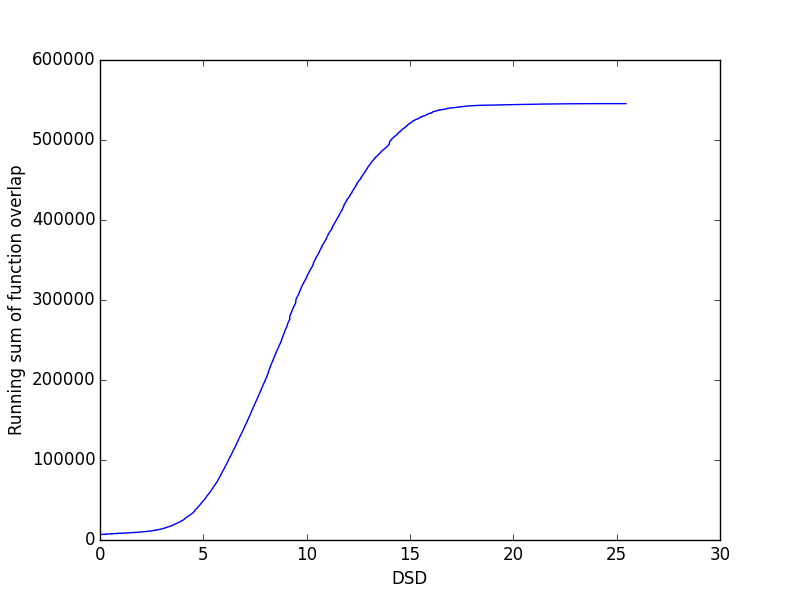
\includegraphics[width=0.5\textwidth]{plots/rat_dsd_running_sum.png}
}
%DSD vs Density Plot:%
\subfloat[DSD vs Density]{
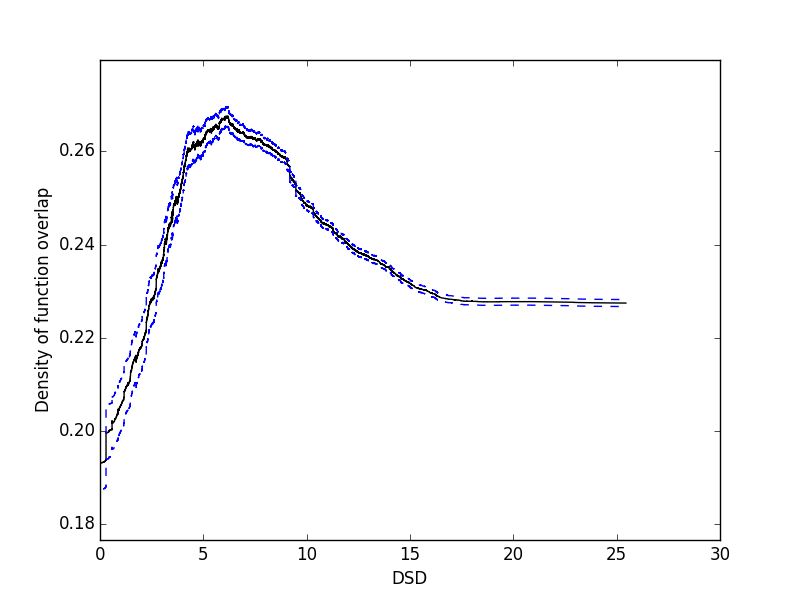
\includegraphics[width=0.5\textwidth]{plots/rat_dsd_density.png}
}}

\centerline{
%DSD vs Pairs Plot:%
\subfloat[DSD vs Pairs]{
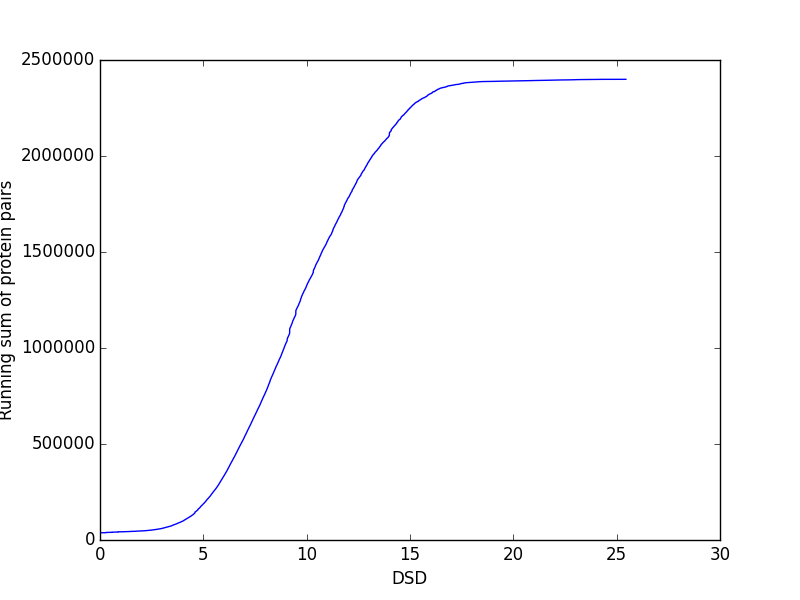
\includegraphics[width=0.5\textwidth]{plots/rat_dsd_pairs.png}
}
% Pairs vs Running Sum %
\subfloat[Pairs vs Running Sum]{
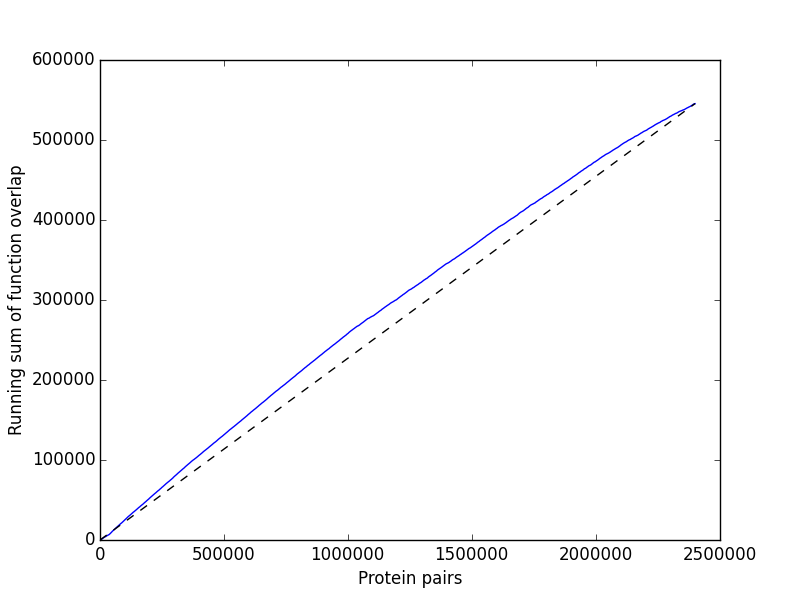
\includegraphics[width=0.5\textwidth]{plots/rat_pairs_running_sum.png}
}}

\end{figure}

\end{document}

 
